\documentclass[a4paper]{extarticle}
\usepackage[utf8]{inputenc}
\usepackage[italian]{babel}
\selectlanguage{italian}
\usepackage[table]{xcolor}
\usepackage{xcolor}
\usepackage{circuitikz}
\usetikzlibrary{positioning, circuits.logic.US}
\usetikzlibrary{shapes.geometric, arrows}
\usetikzlibrary {shapes.gates.logic.US, shapes.gates.logic.IEC, calc}
\tikzset {branch/.style={fill, shape = circle, minimum size = 3pt, inner sep = 0pt}}
\usetikzlibrary{matrix,calc}
\usepackage{multirow}
\usepackage{float}
\usepackage{geometry}
\usepackage{tabularx}
\usepackage{pgf-pie}
\usepackage{tikz}
\usepackage{amsmath}
\usepackage{amssymb}
\usepackage{color, soul}
\usepackage{fancyhdr}
\usepackage{graphicx}
\usepackage{subfig}
\graphicspath{ {./img/} }
\newtheorem{theorem}{Teorema}[section]
\newtheorem{corollary}{Corollario}[theorem]
\newtheorem{lemma}[theorem]{Lemma}

% Specifiche
\geometry{
 a4paper,
 top=20mm,
 left=30mm,
 right=30mm,
 bottom=30mm
}

\nocite{*}

\pagestyle{fancy}
\fancyhf{}
\fancyhead[LO]{\nouppercase{\leftmark}}
\fancyfoot[CE, CO]{\thepage}
\addtolength{\headheight}{1em}
\addtolength{\footskip}{-0.5em}

\newcommand{\quotes}[1]{``#1''}
\renewcommand\tabularxcolumn[1]{>{\vspace{\fill}}m{#1}<{\vspace{\fill}}}
\renewcommand\arraystretch{}
\newcolumntype{P}{>{\centering\arraybackslash}X}

\title{\textbf{Prima prova - A.A. 2021/22\\}}
\author{Cognome e Nome : Piccin Enrico}
\date{Matricola: IN0501089}

\begin{document}

\vspace{-10mm}
\maketitle

%\tableofcontents
%\newpage
\noindent
\section{Esercizio}
Utilizzando una rappresentazione binaria in Fixed Point che utilizzi $4$ bit per la parte intera e $3$ bit per la parte frazionaria, che adotti una notazione \quotes{Signed} e definendo inoltre $\delta$ lo step tra due numeri consecutivi, si rappresenti in decimale ed in binario rispettivamente:
\begin{enumerate}
    \item Il massimo numero positivo rappresentabile
    \[0111.111_2 = 7.875_{10}\]
    \item Il minimo numero negativo
    \[1000.000_2 = -8_{10}\]
    \item Lo step tra due numeri consecutivi $\delta$
    \[0000.001_2 = 0.125_{10}\]
    \item il numero $-\delta$
    \[1111.111_2 = -0.125\]
\end{enumerate}

\noindent
\section{Esercizio}
Su di un bus a $10$ bit viaggiano dei dati codificati secondo il codice di Hamming con h=4.\\
Supponendo che i quattro bit di controllo siano posizionati nelle posizioni $0$ (il bit di parità globale) e successivamente nelle posizioni $1$, $2$, $4$ e $8$ e supponendo di ricevere le seguenti parole (scritte in esagesimale a $10$ bit) analizzare la tipologia di errore eventualmente rilevato e, ove possibile, suggerire la parola originale trasmessa più probabile.
\begin{enumerate}
    \item $0$x$124 = 01 0010 0100$

    \noindent
    \begin{table}[H]
    \rowcolors{1}{white}{white}
    \setlength{\tabcolsep}{4pt}
    \renewcommand{\arraystretch}{1}
    \centering
    \begin{tabular}{|c|c|c|c|c|c|c|c|c|c|}
        \hline
        $0$ & $1$ & $2$ & $3$ & $4$ & $5$ & $6$ & $7$ & $8$ & $9$\\
        \hline
        \cellcolor{orange!75!white}0 & \cellcolor{orange!25!white}1 &\cellcolor{orange!25!white}0 & 0 & \cellcolor{orange!25!white}1 & 0 & 0 & 1 & \cellcolor{orange!25!white}0 & 0\\
        \hline
    \end{tabular}
    \end{table}

    \vspace{1em}
    \noindent
    Controllando i bit di parità si osserva che
    \begin{enumerate}
        \item il bit di parità globale è errato, per cui $b_0=1$;
        \item il bit di parità $b_1$ è corretto;
        \item il bit di parità $b_2$ è sbagliato, per cui $b_2=1$;
        \item il bit di parità $b_4$ è corretto;
        \item il bit di parità $b_8$ è corretto; 
    \end{enumerate}
    Il bit di parità globale indica che si è verificato un errore di molteplicità dispari; essendo molto più probabile l'errore singolo, che triplo, il bit errato potrebbe essere proprio il bit $b_2$.

    \item $0$x$099 = 00 1001 1001$

    \noindent
    \begin{table}[H]
    \rowcolors{1}{white}{white}
    \setlength{\tabcolsep}{4pt}
    \renewcommand{\arraystretch}{1}
    \centering
    \begin{tabular}{|c|c|c|c|c|c|c|c|c|c|}
        \hline
        $0$ & $1$ & $2$ & $3$ & $4$ & $5$ & $6$ & $7$ & $8$ & $9$\\
        \hline
        \cellcolor{orange!75!white}0 & \cellcolor{orange!25!white}0 &\cellcolor{orange!25!white}1 & 0 & \cellcolor{orange!25!white}0 & 1 & 1 & 0 & \cellcolor{orange!25!white}0 & 1\\
        \hline
    \end{tabular}
    \end{table}

    \vspace{1em}
    \noindent
    Controllando i bit di parità si osserva che
    \begin{enumerate}
        \item il bit di parità globale è corretto;
        \item il bit di parità $b_1$ è corretto;
        \item il bit di parità $b_2$ è corretto;
        \item il bit di parità $b_4$ è corretto;
        \item il bit di parità $b_8$ è sbagliato, per cui $b_8=1$; 
    \end{enumerate}
    Il bit di parità globale indica che si è verificato un errore di molteplicità pari; essendo molto più probabile l'errore doppio, che quadruplo, la coppia di bit errati potrebbe essere $b_0$ e $b_8$, oppure $b_1$ e $b_9$.

    \item $0$x$025 = 00 0010 0101$

    \noindent
    \begin{table}[H]
    \rowcolors{1}{white}{white}
    \setlength{\tabcolsep}{4pt}
    \renewcommand{\arraystretch}{1}
    \centering
    \begin{tabular}{|c|c|c|c|c|c|c|c|c|c|}
        \hline
        $0$ & $1$ & $2$ & $3$ & $4$ & $5$ & $6$ & $7$ & $8$ & $9$\\
        \hline
        \cellcolor{orange!75!white}0 & \cellcolor{orange!25!white}0 &\cellcolor{orange!25!white}0 & 0 & \cellcolor{orange!25!white}1 & 0 & 0 & 1 & \cellcolor{orange!25!white}0 & 1\\
        \hline
    \end{tabular}
    \end{table}

    \vspace{1em}
    \noindent
    Controllando i bit di parità si osserva che
    \begin{enumerate}
        \item il bit di parità globale è sbagliato, per cui $b_0=1$;
        \item il bit di parità $b_1$ è corretto;
        \item il bit di parità $b_2$ è sbagliato, per cui $b_2=1$;
        \item il bit di parità $b_4$ è corretto;
        \item il bit di parità $b_8$ è sbagliato, per cui $b_8=1$; 
    \end{enumerate}
    Il bit di parità globale indica che si è verificato un errore di molteplicità dispari; in linea teorica, sarebbe molto più probabile l'errore singolo, che triplo; tuttavia, analizzando la codifica della posizione del'errore si ottiene $1010_2=10_{10}$, ossia un bit che non appartiene alla stringa di bit ricevuta; ciò, pertanto, indica che si è verificato un errore triplo.

    \item $0$x$33F = 11 0011 1111$

    \noindent
    \begin{table}[H]
    \rowcolors{1}{white}{white}
    \setlength{\tabcolsep}{4pt}
    \renewcommand{\arraystretch}{1}
    \centering
    \begin{tabular}{|c|c|c|c|c|c|c|c|c|c|}
        \hline
        $0$ & $1$ & $2$ & $3$ & $4$ & $5$ & $6$ & $7$ & $8$ & $9$\\
        \hline
        \cellcolor{orange!75!white}1 & \cellcolor{orange!25!white}1 &\cellcolor{orange!25!white}0 & 0 & \cellcolor{orange!25!white}1 & 1 & 1 & 1 & \cellcolor{orange!25!white}1 & 1\\
        \hline
    \end{tabular}
    \end{table}

    \vspace{1em}
    \noindent
    Controllando i bit di parità si osserva che
    \begin{enumerate}
        \item il bit di parità globale è corretto;
        \item il bit di parità $b_1$ è corretto;
        \item il bit di parità $b_2$ è corretto;
        \item il bit di parità $b_4$ è corretto;
        \item il bit di parità $b_8$ è corretto.
    \end{enumerate}
    Tutti i bit di parità sono corretti. Ciò indica che molto probabilmente la parola ricevuta è corretta, anche se è possibile che si sia verificato (con probabilità molto bassa) un errore multiplo di $4$ non rilevabile dal codice.
\end{enumerate}

\noindent
\section{Esercizio}
In un codice Ecc3, supponendo che la probabilità di errore su ogni singolo bit sia dello $0.1 \%$, qual è la probabilità di un errore non rilevabile quando si trasmette la cifra \quotes{1}? E se al codice vi si aggiungesse un controllore di parità?

\begin{enumerate}
    \item Essendo il codice Ecc3 un codice non completo in cui la distanza di Hamming (la minima distanza) è pari a $h=1$, la probabilità di un errore non rilevato è
    \[N_h \cdot p^h = 3 \cdot 0.1\% = 0.3\%\]

    \item Introducendo un controllore di parità, la distanza minima tra le parole passa da $h=1$ a $h=2$. Il numero di parole a distanza $h=2$ dalla parola $1$ è pari a $5$, per cui la probabilità di un errore non rilevato è
    \[N_h \cdot p^h = 5 \cdot (0.1\%)^2 = 5 \times 10^{-6}\]
\end{enumerate}

\noindent
\section{Esercizio}
Come si eseguirebbe in \quotes{codice ad eccesso $3$} l'operazione $34-56$ avendo a disposizione solamente \quotes{sommatori}? Esplicitarne tutti i passaggi.

\begin{itemize}
    \item Prima di tutto si codificano in Ecc3 i due valori da \quotes{sommare}:
    \begin{align*}
        &34_{10} = 0110\_0111_{\text{Ecc3}}\\
        &56_{10} = 1000\_1001_{\text{Ecc3}}\\
    \end{align*}

    \item Dopodiché si procede complementando il secondo addendo:
    \[1000\_1001 \hspace{1em} \rightarrow \hspace{1em} 0111\_0110 + 1 = 0111\_0111\]

    \item Ora si procede ad eseguire la somma tra i due valori così ottenuti:
    \noindent
    \begin{table}[H]
    \rowcolors{1}{white}{white}
    \setlength{\tabcolsep}{4pt}
    \renewcommand{\arraystretch}{1}
    \centering
    \begin{tabular}{cc}
        1100 1110 &\\
        \hline
        $0110\_0111$ & +\\
        $0111\_0111$ & =\\
        \hline
        $1101\_1110$
    \end{tabular}
    \end{table}

    \item Si esegue, ora, la correzione del risultato: dal momento che non si è avuto riporto né sul primo né sul secondo digit, si somma $13$ (ovvero si sottrae $3$) ad entrambi
    
    \noindent
    \begin{table}[H]
    \rowcolors{1}{white}{white}
    \setlength{\tabcolsep}{4pt}
    \renewcommand{\arraystretch}{1}
    \centering
    \begin{tabular}{cc}
        0100 0100 &\\
        \hline
        $1101\_1110$ & +\\
        $1101\_1101$ & =\\
        \hline
        $1010\_1011$
    \end{tabular}
    \end{table}

    \item Il valore ottenuto, tuttavia, non è da considerarsi il valore cercato. Questo perché nella somma di partenza non si è ottenuto un riporto sul digit successivo (ossia il $3$ digit) come ci si aspettava a seguito dell'operazione di complementazione. Ciò indica che si è ottenuto un valore negativo, per cui deve essere complementato:
    \[1010\_1011 \hspace{1em} \rightarrow \hspace{1em} 0101\_0100 + 1 = 0101\_0101\]

    \item Ecco che, quindi, si è ottenuto il valore cercato, ossia
    \[- 0101\_0101_{\text{Ecc}3} = -22_{10}\]
\end{itemize}

\noindent
\section{Esercizio}
La funzione composta dai seguenti minterm
\[2, 5, 9, 12 ,13 ,15 ,16 ,18 ,19 ,22 ,26 ,29\]
è simmetrica? In caso affermativo che funzione è?

\begin{itemize}
    \item Per stabilire se la funzione è simmetrica, si scrive

    \noindent
    \begin{table}[H]
    \rowcolors{1}{white}{white}
    \setlength{\tabcolsep}{4pt}
    \renewcommand{\arraystretch}{1}
    \centering
    \begin{tabular}{|c|c|c|}
        minterm & codifica & peso\\
        \hline
        $2$ & $00010$ & 1\\
        $5$ & $00101$ & 2\\
        $9$ & $01001$ & 2\\
        $12$ & $01100$ & 2\\
        $13$ & $01101$ & 3\\
        $15$ & $01111$ & 4\\
        $16$ & $10000$ & 1\\
        $18$ & $10010$ & 2\\
        $19$ & $10011$ & 3\\
        $22$ & $10110$ & 3\\
        $26$ & $11010$ & 3\\
        $29$ & $11101$ & 4\\
        \hline
         & & \\
         & $11111$ & \\
    \end{tabular}
    \end{table}

    \item Pur essendo i rapporti costanti, essi sono unitari e non possono essere discriminati i reciproci. Si procede, quindi, a scomporre la tabella di cui sopra in due sotto-tabelle in cui viene fissata la prima variabile, ottenendo
    
    \noindent
    \begin{table}[H]
    \rowcolors{1}{white}{white}
    \setlength{\tabcolsep}{4pt}
    \renewcommand{\arraystretch}{1}
    \centering
    \begin{tabular}{ccc}
        {
            \begin{tabular}{|c|c|c|}
                minterm & codifica & peso\\
                \hline
                $2$ & $0010$ & 1\\
                $5$ & $0101$ & 2\\
                $9$ & $1001$ & 2\\
                $12$ & $1100$ & 2\\
                $13$ & $1101$ & 3\\
                $15$ & $1111$ & 4\\
                \hline
                & &\\
                 & $22\dfrac{1}{2}2$ & \\
            \end{tabular}
        }&&
        {
            \begin{tabular}{|c|c|c|}
                minterm & codifica & peso\\
                \hline
                $16$ & $0000$ & 0\\
                $18$ & $0010$ & 1\\
                $19$ & $0011$ & 2\\
                $22$ & $0110$ & 2\\
                $26$ & $1010$ & 2\\
                $29$ & $1101$ & 3\\
                \hline
                & & \\
                 & $\dfrac{1}{2}\dfrac{1}{2}2\dfrac{1}{2}$ & \\
            \end{tabular}
        }\\
         && \\
        $x=0$ && $x=1$\\
    \end{tabular}
    \end{table}

    \item dall'analisi dei rapporti appare evidente che il rapporto corrispondente alla terza colonna rappresenta il reciproco del rapporto di tutte le altre. Pertanto, si inverte la terza colonna in ambo le tabelle, ottenendo:
    
    \noindent
    \begin{table}[H]
    \rowcolors{1}{white}{white}
    \setlength{\tabcolsep}{4pt}
    \renewcommand{\arraystretch}{1}
    \centering
    \begin{tabular}{ccc}
        {
            \begin{tabular}{|c|c|c|}
                minterm & codifica & peso\\
                \hline
                $2$ & $0000$ & 0\\
                $5$ & $0111$ & 3\\
                $9$ & $1011$ & 3\\
                $12$ & $1110$ & 3\\
                $13$ & $1111$ & 4\\
                $15$ & $1101$ & 3\\
                \hline
                & & \\
                 & $2222$ & \\
            \end{tabular}
        }&&
        {
            \begin{tabular}{|c|c|c|}
                minterm & codifica & peso\\
                \hline
                $16$ & $0010$ & 1\\
                $18$ & $0000$ & 0\\
                $19$ & $0001$ & 1\\
                $22$ & $0100$ & 1\\
                $26$ & $1000$ & 1\\
                $29$ & $1111$ & 4\\
                \hline
                & & \\
                 & $\dfrac{1}{2}\dfrac{1}{2}\dfrac{1}{2}\dfrac{1}{2}$ & \\
            \end{tabular}
        }\\
         && \\
        $x=0$ && $x=1$\\
    \end{tabular}
    \end{table}

    \item Ora tutti i rapporti sono costanti. Ricostruendo la funzione di partenza, con l'opportuna commutazione, si ottiene
    
    \noindent
    \begin{table}[H]
    \rowcolors{1}{white}{white}
    \setlength{\tabcolsep}{4pt}
    \renewcommand{\arraystretch}{1}
    \centering
    \begin{tabular}{|c|c|c|}
        minterm & codifica & peso\\
        \hline
        $2$ & $00000$ & 0\\
        $5$ & $00111$ & 3\\
        $9$ & $01011$ & 3\\
        $12$ & $01110$ & 3\\
        $13$ & $01111$ & 4\\
        $15$ & $01101$ & 3\\
        $16$ & $10010$ & 2\\
        $18$ & $10000$ & 1\\
        $19$ & $10001$ & 2\\
        $22$ & $10100$ & 2\\
        $26$ & $11000$ & 2\\
        $29$ & $11111$ & 5\\
        \hline
         & & \\
         & $11111$ & \\
    \end{tabular}
    \end{table}

    \vspace{1em}
    \noindent
    Appare evidente che il numero delle righe per ogni livello di simmetria non risulta essere congruo con quello previsto per una funzione simmetrica dato dal valore
    \[\binom{n}{k}\]
    Tuttavia, scomponendo la tabella rispetto a $x$ si aveva una corrispondenza esatta per quanto riguarda il numero di righe per ogni livello di simmetria. Ciò, suggerisce, la possibilità di commutare anche la prima colonna, ottenendo

    \noindent
    \begin{table}[H]
    \rowcolors{1}{white}{white}
    \setlength{\tabcolsep}{4pt}
    \renewcommand{\arraystretch}{1}
    \centering
    \begin{tabular}{|c|c|c|}
        minterm & codifica & peso\\
        \hline
        $2$ & $10000$ & 1\\
        $5$ & $10111$ & 4\\
        $9$ & $11011$ & 4\\
        $12$ & $11110$ & 4\\
        $13$ & $11111$ & 5\\
        $15$ & $11101$ & 4\\
        $16$ & $00010$ & 1\\
        $18$ & $00000$ & 0\\
        $19$ & $00001$ & 1\\
        $22$ & $00100$ & 1\\
        $26$ & $01000$ & 1\\
        $29$ & $01111$ & 4\\
        \hline
         & & \\
         & $11111$ & \\
    \end{tabular}
    \end{table}

    \item Naturalmente i rapporti permangono costanti, come costanti saranno anche i rapporti individuati nelle sotto-tabelle date dalla decomposizione di $f$ rispetto a $x$.\\
    Complementando $x$, tuttavia, non solo i rapporti sono quelli attesi, ma anche il numero di righe per ogni livello di simmetria, infatti:
    \begin{itemize}
        \item per il livello $k=0$ si hanno $\displaystyle{\binom{5}{0}}=1$ termini;
        \item per il livello $k=1$ si hanno $\displaystyle{\binom{5}{1}}=5$ termini;
        \item per il livello $k=4$ si hanno $\displaystyle{\binom{5}{4}}=5$ termini;
        \item per il livello $k=5$ si hanno $\displaystyle{\binom{5}{5}}=1$ termini;
    \end{itemize}

    \item Ad ulteriore riprova, si suddivide la tabella di partenza raggruppando i termini con lo stesso peso $k$:

    \noindent
    \begin{table}[H]
    \rowcolors{1}{white}{white}
    \setlength{\tabcolsep}{4pt}
    \renewcommand{\arraystretch}{1}
    \centering
    \begin{tabular}{ccc}
        {
            \begin{tabular}{|c|c|c|}
                minterm & codifica & peso\\
                \hline
                $18$ & $00000$ & 0\\
                \hline
                & & \\
                & $0000$ & \\
            \end{tabular}
        }&&
        {
            \begin{tabular}{|c|c|c|}
                minterm & codifica & peso\\
                \hline
                $2$  & $10000$ & 1\\
                $16$ & $00010$ & 1\\
                $19$ & $00001$ & 1\\
                $22$ & $00100$ & 1\\
                $26$ & $01000$ & 1\\
                \hline
                & & \\
                & $\dfrac{1}{4}\dfrac{1}{4}\dfrac{1}{4}\dfrac{1}{4}$ & \\
            \end{tabular}
        }
    \end{tabular}
    \end{table}

    \vspace{2em}
    \noindent
    \begin{table}[H]
    \rowcolors{1}{white}{white}
    \setlength{\tabcolsep}{4pt}
    \renewcommand{\arraystretch}{1}
    \centering
    \begin{tabular}{ccc}
        {
            \begin{tabular}{|c|c|c|}
                minterm & codifica & peso\\
                \hline
                $5$  & $10111$ & 4\\
                $9$  & $11011$ & 4\\
                $12$ & $11110$ & 4\\
                $15$ & $11101$ & 4\\
                $29$ & $01111$ & 4\\
                \hline
                & & \\
                & $44444$ & \\
            \end{tabular}
        }
        &&
        {
            \begin{tabular}{|c|c|c|}
                minterm & codifica & peso\\
                \hline
                $13$ & $11111$ & 5\\
                \hline
                & & \\
                & $\infty\infty\infty\infty\infty$ & \\
            \end{tabular}
        }
    \end{tabular}
    \end{table}

    \vspace{1em}
    \noindent
    Infatti, come ci si aspettava
    \begin{itemize}
        \item per il livello $k=0$, il rapporto atteso è $\dfrac{0}{5-0}=0$;
        \item per il livello $k=1$, il rapporto atteso è $\dfrac{1}{5-1}=\dfrac{1}{4}$;
        \item per il livello $k=4$, il rapporto atteso è $\dfrac{4}{5-4}=4$;
        \item per il livello $k=5$, il rapporto atteso è $\dfrac{5}{5-5}=\infty$;
    \end{itemize}    
    
    \item Pertanto si è ottenuta la funzione simmetrica
    \[S^{5}_{\{0,1,4,5\}}(\overline{x},y,z,\overline{w},u)\]
\end{itemize}

\noindent
\section{Esercizio}
Fornire una realizzazione della funzione di cui all'esercizio $5$.

\begin{itemize}
    \item Essendo la funzione simmetrica esaminata a $5$ variabili, sarà sufficiente considerare un sommatore che produca in uscita $3$ bit sufficienti per codificare i pesi da $0$ a $5$. Successivamente, con una logica opportuna, si andranno a prendere in considerazione i bit di somma per produrre l'uscita della funzione.
    
    \item Lo schema cercato è il seguente:

    \begin{figure}[H]
        \centering
        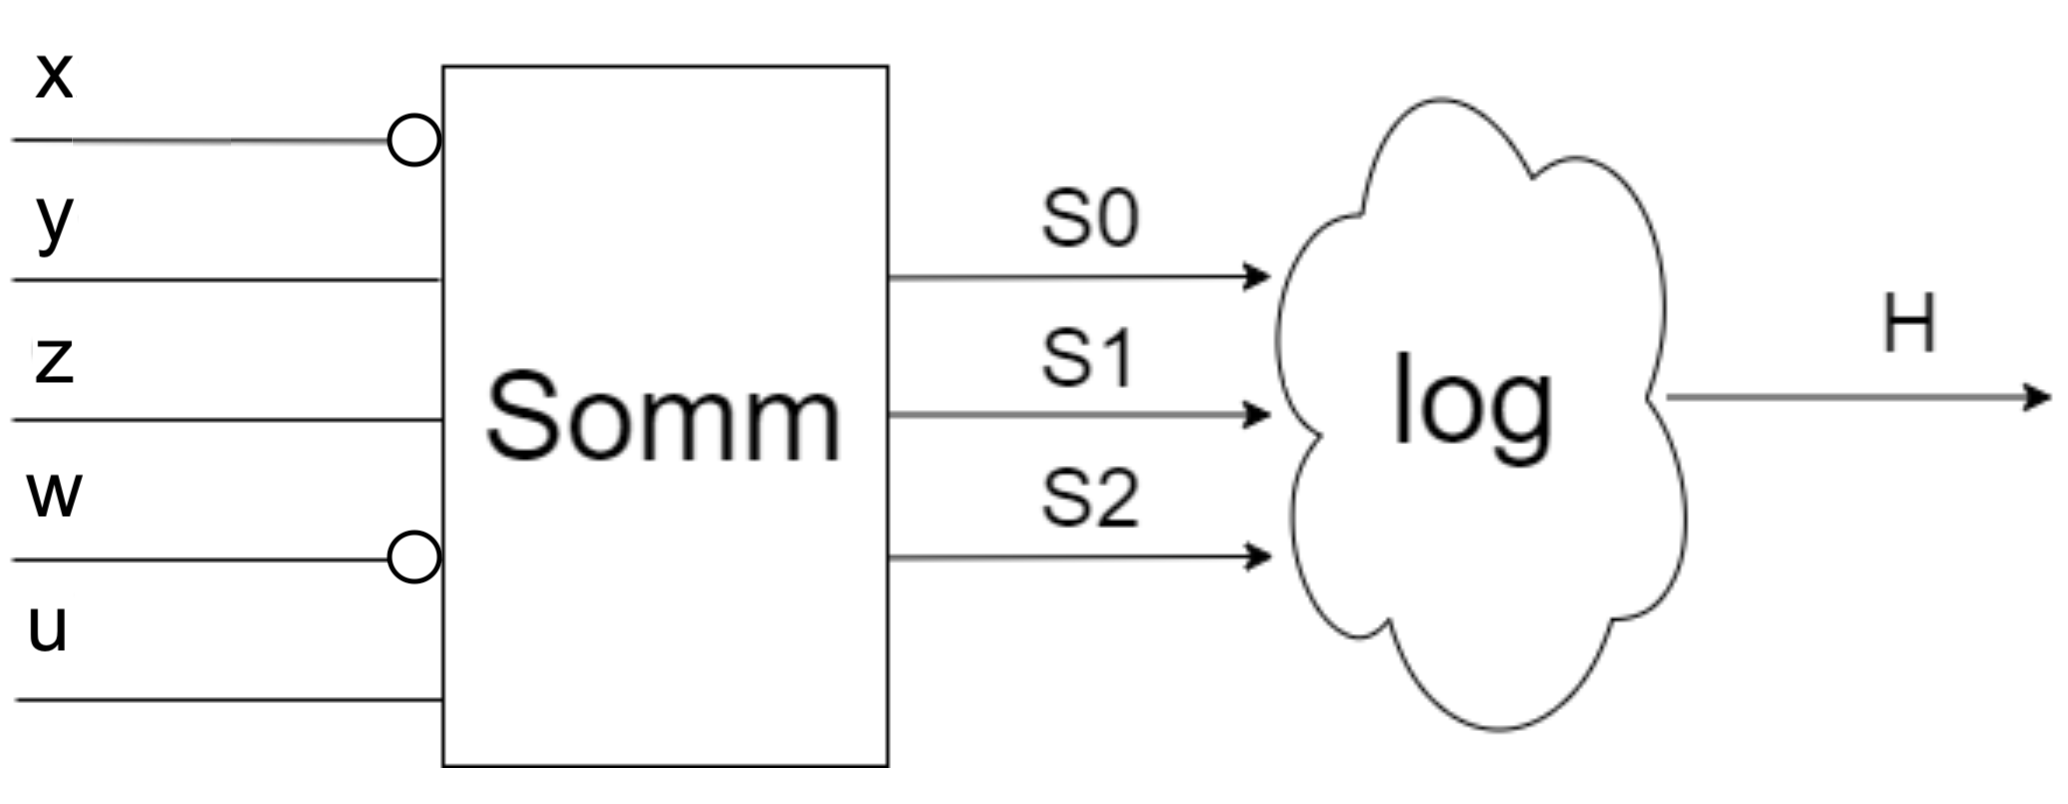
\includegraphics[width=0.5\textwidth]{logica-realizzazione-funzione-simmetrica.png}
        \caption{Logica di realizzazione della funzione simmetrica}
        \label{fig:logica_realizzazione_funzione_simmetrica}
    \end{figure}

    \item Per la realizzazione del sommatore sarà sufficiente ricorrere a $2$ full-adder e ad un half-adder, come mostrato nel seguito:
    
    \begin{figure}[H]
        \centering
        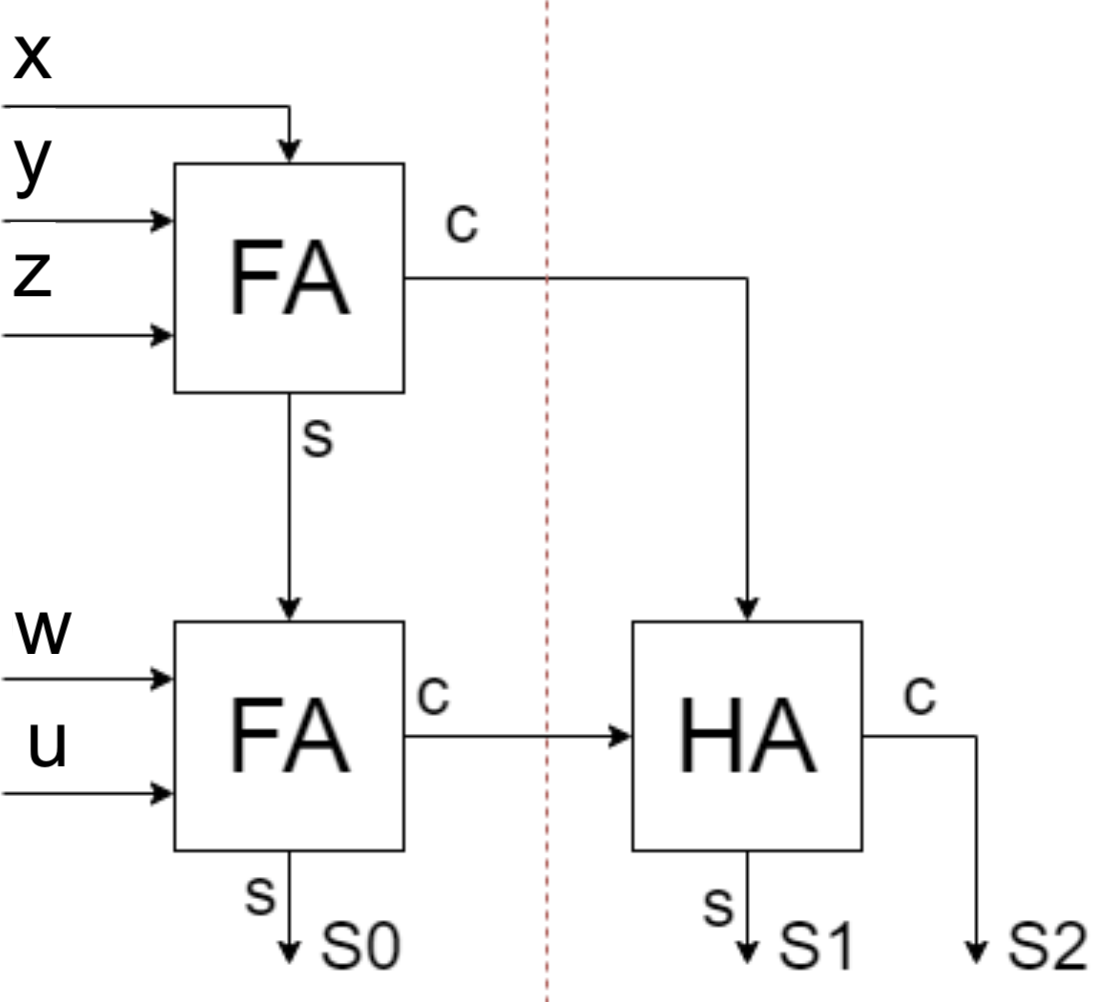
\includegraphics[width=0.5\textwidth]{sommatore-calcolo-peso-parola.png}
        \caption{Sommatore per il calcolo del peso della parola}
        \label{fig:sommatore_calcolo_peso_parola}
    \end{figure}
    
    \item Dal momento che si necessita di realizzare una funzione simmetrica che produce in uscita il valore $1$ in corrispondenza dei pesi $0,1,4,5$, si realizza la mappa seguente

    \noindent
    \begin{table}[H]
        \rowcolors{1}{white}{white}
        \setlength{\tabcolsep}{4pt}
        \renewcommand{\arraystretch}{1}
        \centering
        \begin{tabular}{|c|c|c|c|c|}
            $S_1S_0$\\
            $S_2$ & $00$ & $01$ & $11$ & $10$\\
            \hline
            $0$ & $1$ & $1$ & $0$ & $0$\\
            $1$ & $1$ & $1$ & $-$ & $-$\\
        \end{tabular}
    \end{table}

    \item Pertanto, la logica di uscita è semplicemente $\overline{S_1}$.
\end{itemize}

\noindent
\section{Esercizio}
Analizzando la funzione in 5 variabili composta dai seguenti termini minimi, secondo una mappa di decomposizione che ponga in evidenza la variabili $x_1$ e $x_3$ come variabili indipendenti, quale decomposizione vi si riconosce ? Evidenziarne le sotto-funzioni che la compongono
\[0,4,8,9,12,13,16,21,22,23,24,25,30,31\]

\begin{itemize}
    \item Si realizza la mappa di decomposizione richiesta

    \noindent
    \begin{table}[H]
    \rowcolors{1}{white}{white}
    \setlength{\tabcolsep}{4pt}
    \renewcommand{\arraystretch}{1}
    \centering
    \begin{tabular}{|c|c|c|c|c|c|c|c|c|c}
        $x_1x_3$ &&&&&&&&\\
        $x_2x_4x_5$  & $000$ & $001$ & $010$ & $011$ & $100$ & $101$ & $110$ & $111$ \\
        \hline
        $00$ & \cellcolor{orange!25!white}$0$ & $1$ & $2$ & $3$ & \cellcolor{orange!25!white}$8$ & \cellcolor{orange!25!white}$9$ & $10$ & $11$ & $f$\\
        $01$ & \cellcolor{orange!25!white}$4$ & $5$ & $6$ & $7$ & \cellcolor{orange!25!white}$12$ &\cellcolor{orange!25!white} $13$ & $14$ & $15$ & $f$\\
        $10$ & \cellcolor{orange!25!white}$16$ & $17$ & $18$ & $19$ & \cellcolor{orange!25!white}$24$ & \cellcolor{orange!25!white}$25$ & $26$ & $27$ & $f$\\
        $11$ & $20$ &\cellcolor{orange!25!white} $21$ &\cellcolor{orange!25!white} $22$ & \cellcolor{orange!25!white}$23$ & $28$ & $29$ & \cellcolor{orange!25!white}$30$ & \cellcolor{orange!25!white}$31$ & $\overline{f}$\\
        \hline 
        &$\overline{g}$& $g$ & $g$ & $g$ & $\overline{g}$ & $\overline{g}$ & $g$ & $g$\\ 
    \end{tabular}
    \end{table}

    \item Si osserva immediatamente la presenza di una funzione $f$ e della sua commutazione $\overline{f}$, così come della funzione $g$ e della sua commutazione $\overline{g}$, descritte come
    \begin{itemize}
        \item $f=x_2\overline{x_4} + \overline{x_4}\overline{x_5}$
        \item $g=x_1 x_3$
    \end{itemize}
    Considerando la funzione $f$, si ottiene
    
    \noindent
    \begin{table}[H]
    \rowcolors{1}{white}{white}
    \setlength{\tabcolsep}{4pt}
    \renewcommand{\arraystretch}{1}
    \centering
    \begin{tabular}{|c|c|c|}
        $f$ & &\\
        $x_1x_3$ & $0$ & $1$\\
        \hline 
        $00$ & $0$ & $1$\\
        $01$ & $0$ & $1$\\
        $10$ & $0$ & $1$\\
        $11$ & $1$ & $0$\\
    \end{tabular}
    \end{table}

    \item All'interno della tabella di cui sopra, però, si riconosce anche la funzione $g$, precedentemente individuata, ovvero
    
    \noindent
    \begin{table}[H]
    \rowcolors{1}{white}{white}
    \setlength{\tabcolsep}{4pt}
    \renewcommand{\arraystretch}{1}
    \centering
    \begin{tabular}{|c|c|c|}
        $f$ & &\\
        $x_1x_3$ & $0$ & $1$\\
        \hline 
        $00$ & $0$ & $1$\\
        $01$ & $0$ & $1$\\
        $10$ & $0$ & $1$\\
        $11$ & $1$ & $0$\\
        \hline
        &$g$ & $\overline{g}$\\
    \end{tabular}
    \end{table}

    \item e riscrivendo una nuova tabella in funzione di $f$ e $g$ si ottiene
    
    \noindent
    \begin{table}[H]
    \rowcolors{1}{white}{white}
    \setlength{\tabcolsep}{4pt}
    \renewcommand{\arraystretch}{1}
    \centering
    \begin{tabular}{|c|c|c|}
        $f$ & &\\
        $g$ & $0$ & $1$\\
        \hline 
        $0$ & $0$ & $1$\\
        $1$ & $1$ & $0$\\
        \hline
        &$g$ & $\overline{g}$\\
    \end{tabular}
    \end{table}

    \noindent
    ossia uno XOR tra $f$ e $g$.

    \item Per cui è immediata la decomposizione seguente
    \[f \oplus g = (x_2\overline{x_4} + \overline{x_4}\overline{x_5}) \oplus (x_1 x_3)\]
\end{itemize}

\noindent
\section{Esercizio}
Il Numero a 12 bit espresso in esagesimale come $0$x$2BC$ quanto vale in Decimale? Secondo quale algoritmo esso può essere convertito in BCD (riportare la procedura in bella copia).

\begin{itemize}
    \item Il numero esagesimale $0$x$2BC$ in binario vale $0010 1011 1100_{2}$, per cui in decimale il suo valore è $700_{10}$;
    \item Per convertirlo tale numero da binario a BCD, si impiega l'algoritmo seguente
    \noindent
    \begin{table}[H]
        \rowcolors{1}{white}{white}
        \setlength{\tabcolsep}{4pt}
        \renewcommand{\arraystretch}{1}
        \centering
        \begin{tabular}{|cccc|cccc|cccc|cccccccccccc}
            &&&&&&&&&&&&$0$&$0$&$1$&$0$&$1$&$0$&$1$&$1$&$1$&$1$&$0$&$0$\\
            &&&&&&&&&&&$0$&$0$&$1$&$0$&$1$&$0$&$1$&$1$&$1$&$1$&$0$&$0$&\\
            &&&&&&&&&&$0$&$0$&$1$&$0$&$1$&$0$&$1$&$1$&$1$&$1$&$0$&$0$&&\\
            &&&&&&&&&$0$&$0$&$1$&$0$&$1$&$0$&$1$&$1$&$1$&$1$&$0$&$0$&&&\\
            &&&&&&&&$0$&$0$&$1$&$0$&$1$&$0$&$1$&$1$&$1$&$1$&$0$&$0$&&&&\\
            &&&&&&&$0$&\cellcolor{cyan!25!white}$0$&\cellcolor{cyan!25!white}$1$&\cellcolor{cyan!25!white}$0$&\cellcolor{cyan!25!white}$1$&$0$&$1$&$1$&$1$&$1$&$0$&$0$&&&&\\
            &&&&&&&&\cellcolor{cyan!25!white}$0$\cellcolor{cyan!25!white}&\cellcolor{cyan!25!white}$0$&\cellcolor{cyan!25!white}$1$&\cellcolor{cyan!25!white}$1$&&&&&&&&&&&&\\
    
            &&&&&&&$0$&$1$&$0$&$0$&$0$&$0$&$1$&$1$&$1$&$1$&$0$&$0$&&&&&\\
            &&&&&&$0$&$1$&$0$&$0$&$0$&$0$&$1$&$1$&$1$&$1$&$0$&$0$&&&&&&\\
            &&&&&$0$&$1$&$0$&$0$&$0$&$0$&$1$&$1$&$1$&$1$&$0$&$0$&&&&&&&\\
            &&&&&$0$&$1$&$0$&$0$&$0$&$0$&$1$&$1$&$1$&$1$&$0$&$0$&&&&&&&\\
            &&&&$0$&$1$&$0$&$0$&$0$&$0$&$1$&$1$&$1$&$1$&$0$&$0$&&&&&&&&\\
            &&&$0$&\cellcolor{cyan!25!white}$1$&\cellcolor{cyan!25!white}$0$&\cellcolor{cyan!25!white}$0$&\cellcolor{cyan!25!white}$0$&\cellcolor{cyan!25!white}$0$&\cellcolor{cyan!25!white}$1$&\cellcolor{cyan!25!white}$1$&\cellcolor{cyan!25!white}$1$&$1$&$0$&$0$&&&&&&&&&\\
    
            &&&&\cellcolor{cyan!25!white}$0$\cellcolor{cyan!25!white}&\cellcolor{cyan!25!white}$0$&\cellcolor{cyan!25!white}$1$&\cellcolor{cyan!25!white}$1$&\cellcolor{cyan!25!white}$0$\cellcolor{cyan!25!white}&\cellcolor{cyan!25!white}$0$&\cellcolor{cyan!25!white}$1$&\cellcolor{cyan!25!white}$1$&&&&&&&&&&&&\\
    
            &&&$0$&$1$&$0$&$1$&$1$&$1$&$0$&$1$&$0$&$1$&$0$&$0$&&&&&&&&&\\
            &&$0$&$1$&\cellcolor{cyan!25!white}$0$&\cellcolor{cyan!25!white}$1$&\cellcolor{cyan!25!white}$1$&\cellcolor{cyan!25!white}$1$&\cellcolor{cyan!25!white}$0$&\cellcolor{cyan!25!white}$1$&\cellcolor{cyan!25!white}$0$&\cellcolor{cyan!25!white}$1$&$0$&$0$&&&&&&&&&&\\
    
            &&&&\cellcolor{cyan!25!white}$0$\cellcolor{cyan!25!white}&\cellcolor{cyan!25!white}$0$&\cellcolor{cyan!25!white}$1$&\cellcolor{cyan!25!white}$1$&\cellcolor{cyan!25!white}$0$\cellcolor{cyan!25!white}&\cellcolor{cyan!25!white}$0$&\cellcolor{cyan!25!white}$1$&\cellcolor{cyan!25!white}$1$&&&&&&&&&&&&\\
    
            &&$0$&$1$&$1$&$0$&$1$&$0$&$1$&$0$&$0$&$0$&$0$&$0$&&&&&&&&&&\\
            &$0$&$1$&$1$&\cellcolor{cyan!25!white}$0$&\cellcolor{cyan!25!white}$1$&\cellcolor{cyan!25!white}$0$&\cellcolor{cyan!25!white}$1$&$0$&$0$&$0$&$0$&$0$&&&&&&&&&&&\\
            &&&&\cellcolor{cyan!25!white}$0$\cellcolor{cyan!25!white}&\cellcolor{cyan!25!white}$0$&\cellcolor{cyan!25!white}$1$&\cellcolor{cyan!25!white}$1$&&&&&&&&&&&&&&&&\\
            &$0$&$1$&$1$&$1$&$0$&$0$&$0$&$0$&$0$&$0$&$0$&$0$&&&&&&&&&&\\
            $0$&$1$&$1$&$1$&$0$&$0$&$0$&$0$&$0$&$0$&$0$&$0$&&&&&&&&&&&\\
            
        \end{tabular}
        \end{table}

        \item Si ottiene, quindi, il numero cercato $0111\_0000\_0000_{\text{BCD}} = 700_{10}$.
    \end{itemize}

\noindent
\section{Dichiarazione}
Il lavoro di cui sopra è stato svolto da me in completa autonomia.
\end{document}